\documentclass[11pt]{article}
\usepackage{amsfonts, amsmath, amssymb}
\usepackage{dcolumn, multirow}
\usepackage{setspace}
\usepackage{epsfig, subfigure, subfloat, graphicx}
\usepackage{tabularx}
\usepackage{anysize, indentfirst, setspace}
\usepackage{verbatim, rotating, paralist}
\usepackage{latexsym}
\usepackage{amsthm}
\usepackage{fullpage}
\usepackage{longtable}
\usepackage{graphicx}
\usepackage{mathabx}
\usepackage{txfonts}
\usepackage{amsfonts}
\usepackage{parskip}
\usepackage{stmaryrd}
\usepackage{color}
\usepackage{mathrsfs}
\usepackage{dsfont}
\usepackage{comment}
\usepackage{url}
\usepackage{rotating}
\usepackage{appendix}
\usepackage{natbib}
\usepackage{tablefootnote}
\usepackage{hyperref}
\usepackage{multicol}
\setlength{\columnsep}{1cm}
\usepackage{enumitem}
\usepackage{ccicons}
\setlist[itemize]{noitemsep, topsep=0pt}
\setlist[enumerate]{noitemsep, topsep=0pt}
\usepackage[margin=2.5cm]{geometry}

\title{Where on Earth are We? \\ Projections and Coordinate Reference Systems}
\author{Nick Eubank\footnote{\href{mailto:nick@nickeubank.com}{nick@nickeubank.com}. Distributed Under a \href{https://creativecommons.org/licenses/by-nc/4.0/}{Creative Commons Attribution - Non-Commercial License \ccbync}}}
\date{\today}

\begin{document}
\maketitle

If I told you that there was a treasure chest buried at the coordinates $(2, 5)$, your first response might be excitement. But your second response would probably be confusion. What on earth do the coordinates $(2, 5)$ mean? Presumably this implies there exists a point $(0, 0)$, and that the treasure is 2 units in the  direction of the positive x-axis and 5 in the direction of the positive y-axis, but where is $(0,0)$, in what direction is the positive x-axis, and is it 2 feet in that direction or two miles?

Relating raw coordinates in an abstract x-y plane to actual places on the earth requires two distinct things: a model of the real, three dimensional globe (Earth), and a specification for how we convert our representations of locations on a roughly spherical object into a 2-dimensional representation.

In this handout, I will refer to these two things as our ``Global Model'' and our ``Flattening Function.'' I'm making up my own terms because there is ZERO consistency in how these things are named across applications in the world of GIS, and I think these are most descriptive. Below I will discuss what terms are used in different contexts, like in R, Python, or ArcGIS.


\section{Globe Model}

Many GIS users are surprised to learn that when two sources provide the same latitude and longitude, those may not always correspond to the same real world location. The reason for this is the location of a real-world point in terms of latitude and longitude depends on the model of the Earth one is using to compute latitudes and longitudes. These models vary, especially in the degree to which they simplify the shape of the Earth -- some assume that the earth is a perfect sphere; some assume it's a almost a sphere, but is a little fat in the middle (an ellipsoid); and some try to capture every hill and valley on the earth.

You can think of the differences between Globe Models as being analogous to differences in globes you've actually seen in your life -- some are perfect balls, while others are spheres with elevations, while others capture the full weirdness of the earth's shape.

\begin{figure}[h!]
	\begin{center}
		\textbf{Different Globe Models}\\
		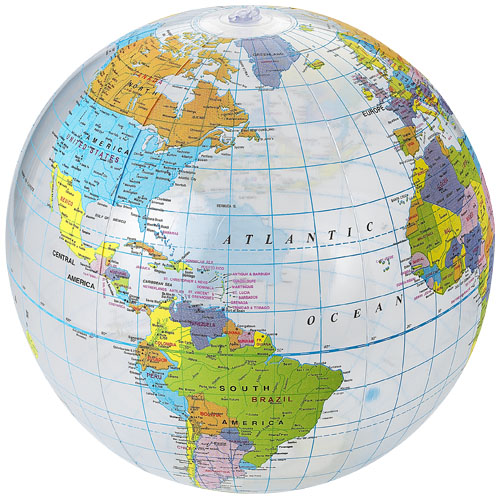
\includegraphics[width = 0.3\textwidth]{media/globe_perfectsphere.jpg} \hspace{0.5cm}
		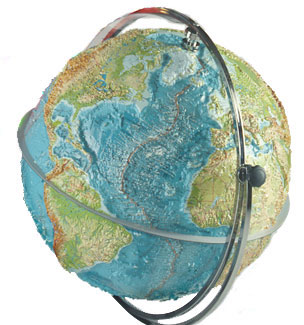
\includegraphics[width = 0.3\textwidth]{media/globe_elevations2.jpg}  \hspace{0.5cm}
		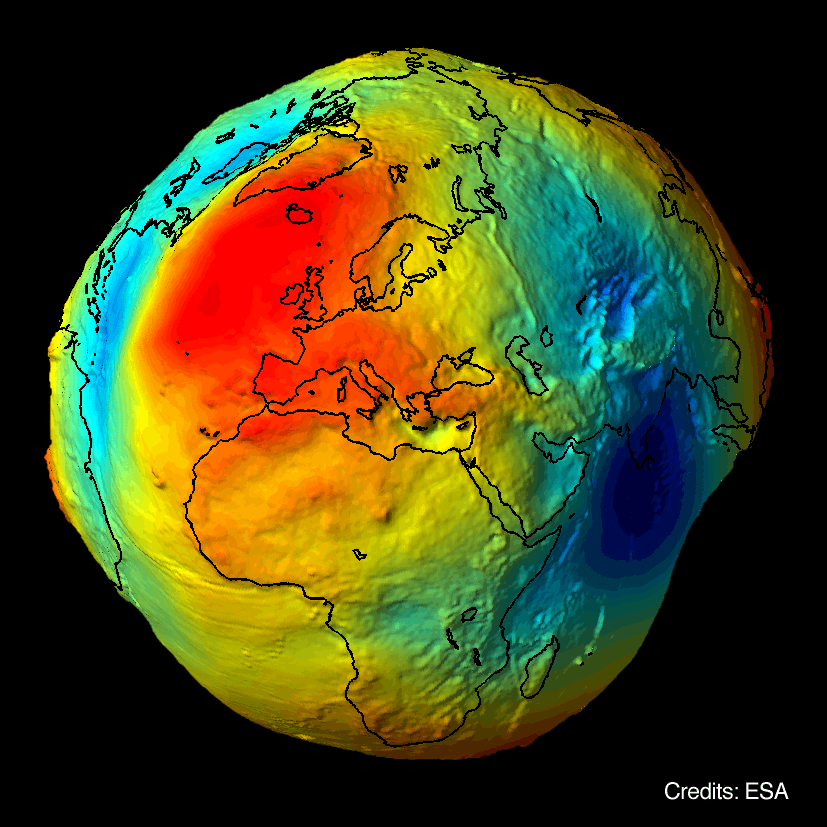
\includegraphics[width = 0.3\textwidth]{media/globe_fullgeoid.png}  \\
		\emph{Smooth sphere} \hspace{2.3cm} \emph{Sphere with elevations} \hspace{2cm} \emph{Satellite-based model of earth}\footnotemark{}
	\end{center}
\end{figure}
 \footnotetext{Note that elevation differences in this figure are exaggerated for visualization.}

One nuance is that Globe Models often have two internal components -- sometimes you may just see a globe model named (the most common is \texttt{WGS84}), but in other settings you may find the Globe Model characterized by \emph{two} parameters -- an ``ellps'' and a ``datum''.\footnote{For the interested party: the ``ellps'' defines the perfect geometric shape that is used as a baseline -- usually either a perfect sphere or an ellipsoid that's like a sphere but a little fatter around the equator -- and the ``datum'' defines the deviations from this perfect shape (like a mountain or valley) at each point on the Earth.} Don't worry about it -- it's still the pair that fully defines a Globe Model.


\section{Flattening Function}
The Earth is round, but our computer screens are not. As a result, before working with spatial data, we have to find a way of taking points on a three-dimensional surface (the Earth) and projecting them onto a two-dimensional surface (our screens).\footnote{A careful reader may ask why this is necessary -- after all, computers can work with 3-D models, why not do everything in three dimensions? The answer is that three dimensions is much harder computationally, and usually if we want to visualize things on a screen, 2-D works best. But there are tools that will do calculations on a sphere, such as calculating distances using ``Great Circle'' routes.} So to work in two-dimensions, we need a Flattening Function.

The thing to remember about Flattening Functions is that \emph{all Flattening Functions are distortions}, so when it comes time to doing an analysis, \textbf{there is no such thing as the ``correct'' Flattening Function} -- different Flattening Function just distort things in different ways.\footnote{OK, so some Flattening Function are more ``right'' than others -- you wouldn't want to use a projection designed to minimize distortions when mapping the United States to project data from Indonesia. But you get the idea.} In particular, no Flattening Function can ever preserve all of the following properties, so you have to pick a Flattening Function that strikes the balance between the various properties you care about most:
\begin{itemize}
	\item Shape\footnote{Or more specifically, the angle at which lines intersect.}
	\item Area
	\item Distances between points
	\item Directions
\end{itemize}

A few examples of Flattening Function (referred to here as Map Projections -- more on nomenclature below) are presented in Figure~\ref{xkcd} below, along with a little commentary from XKCD.

\begin{figure}[h!]
	\begin{center}
		\caption{}\label{xkcd}
		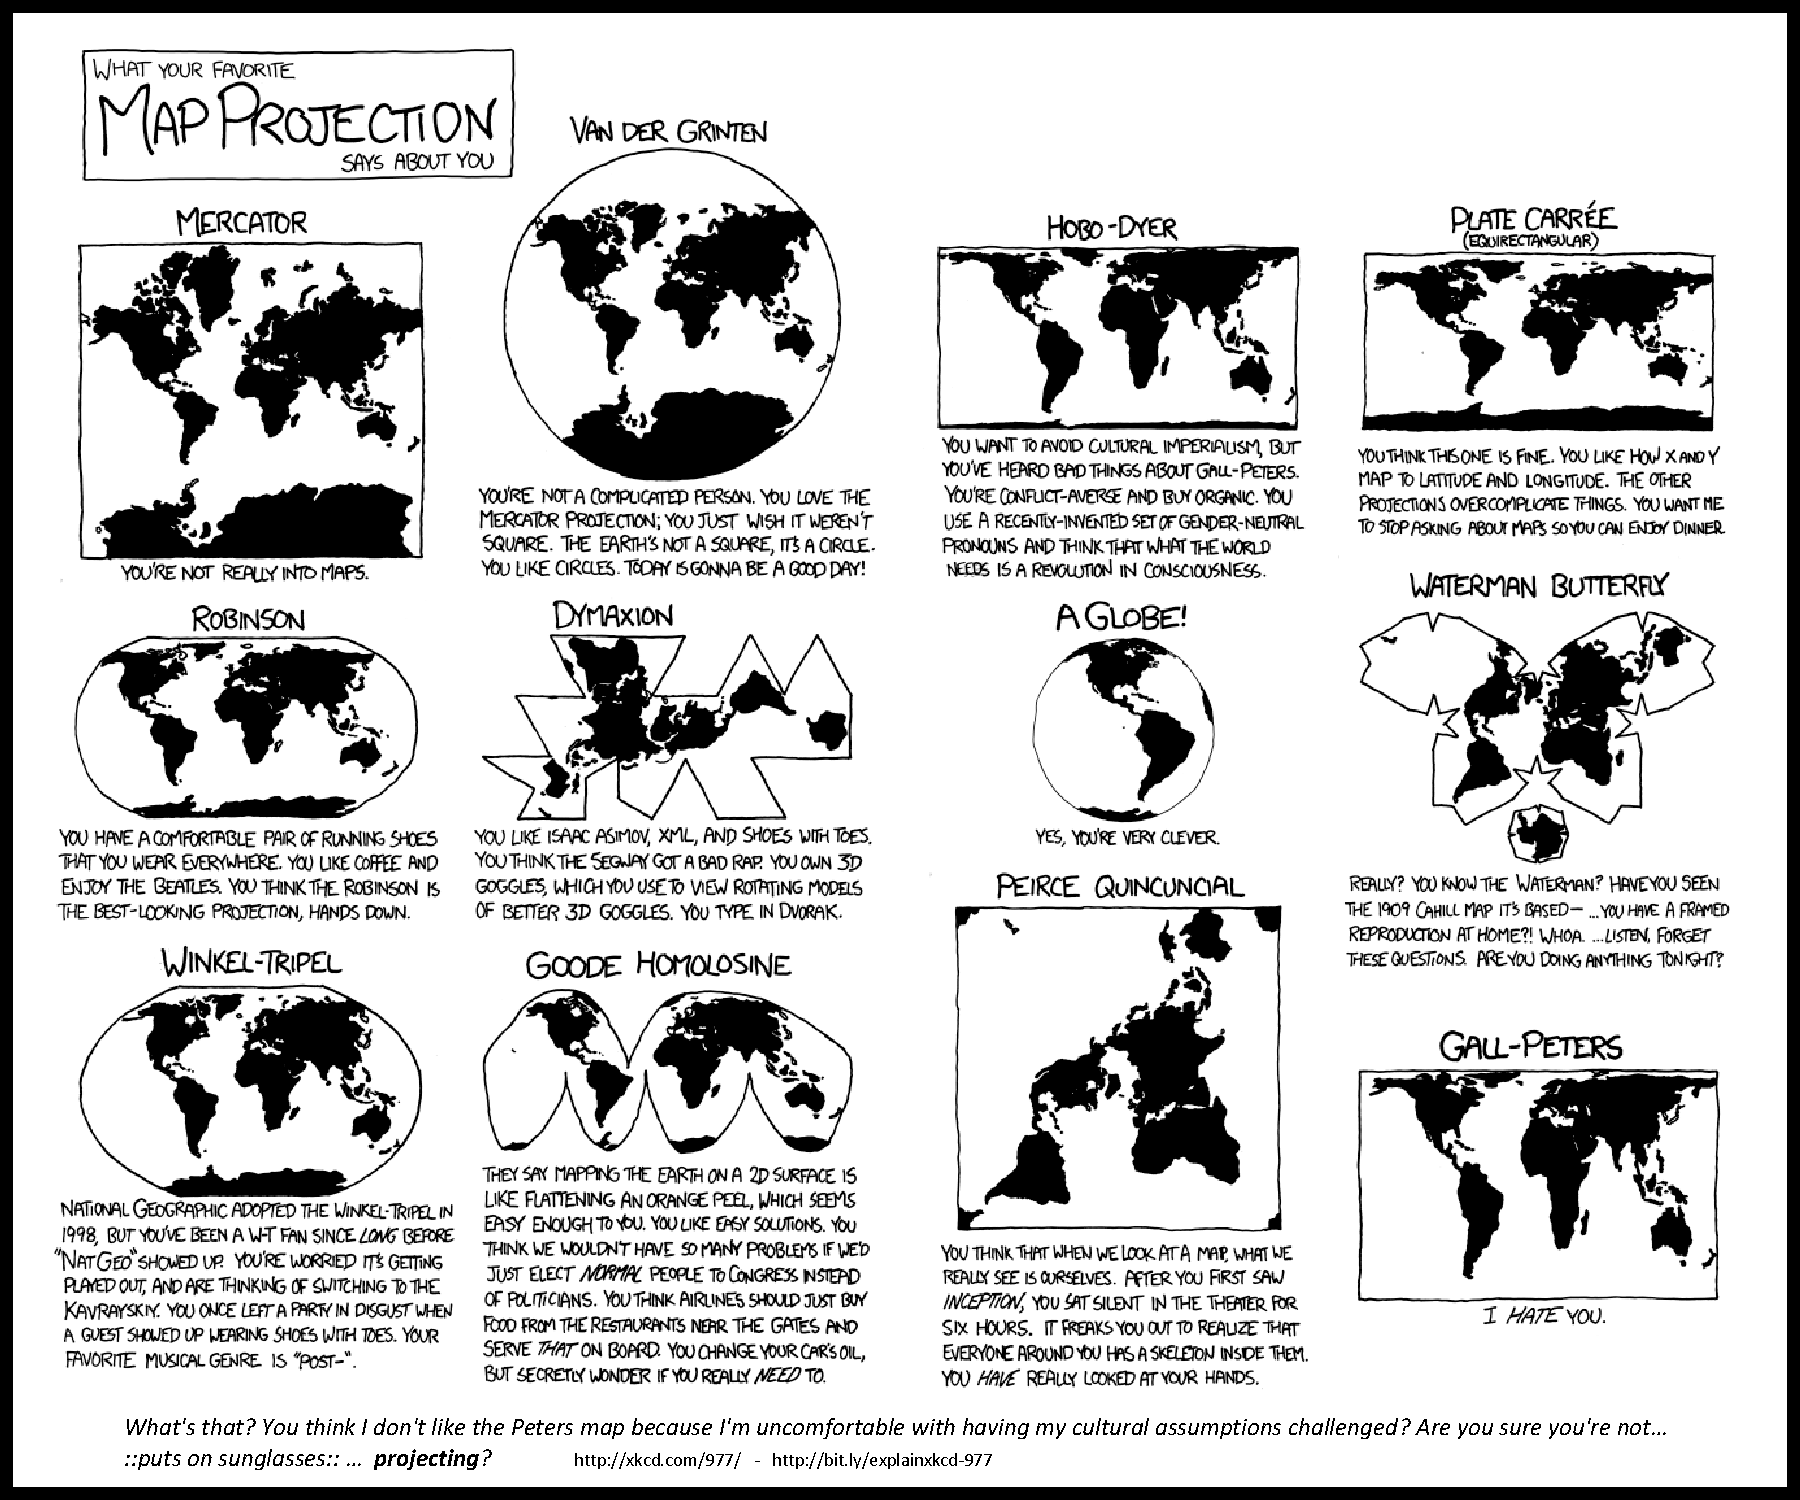
\includegraphics[width = \textwidth]{media/xkcd_projections.pdf}
	\end{center}
\end{figure}

\subsection{Combining Globe Models and Flattening Functions}

If you are working with spatial data in two-dimensions (which is almost always the case unless you've gone out of your way to use some obscure software that tries to treat the Earth as a globe), you are {\color{red}always} using both a Globe Model and a Flattening Function, {\color{red} even if you don't realize it.}

This can be a source of immense confusion. For example, if you have data in units of latitude and longitude (which correspond to locations on a Globe and were collected with a specific Globe Model in mind), you may \emph{think} you aren't using a Flattening Function. After all, since latitude and longitude are defined as locations on a sphere, aren't use working on the sphere?

No. What's happening is that you are treating latitude and longitude as x-y coordinates in a two-dimensional plane, which means you are implicitly applying a Plate Carr\'ee Flattening Function, which looks like:

\begin{figure}
	\centering
	\caption{Plate Carr\'ee Flattening Function}\label{}
	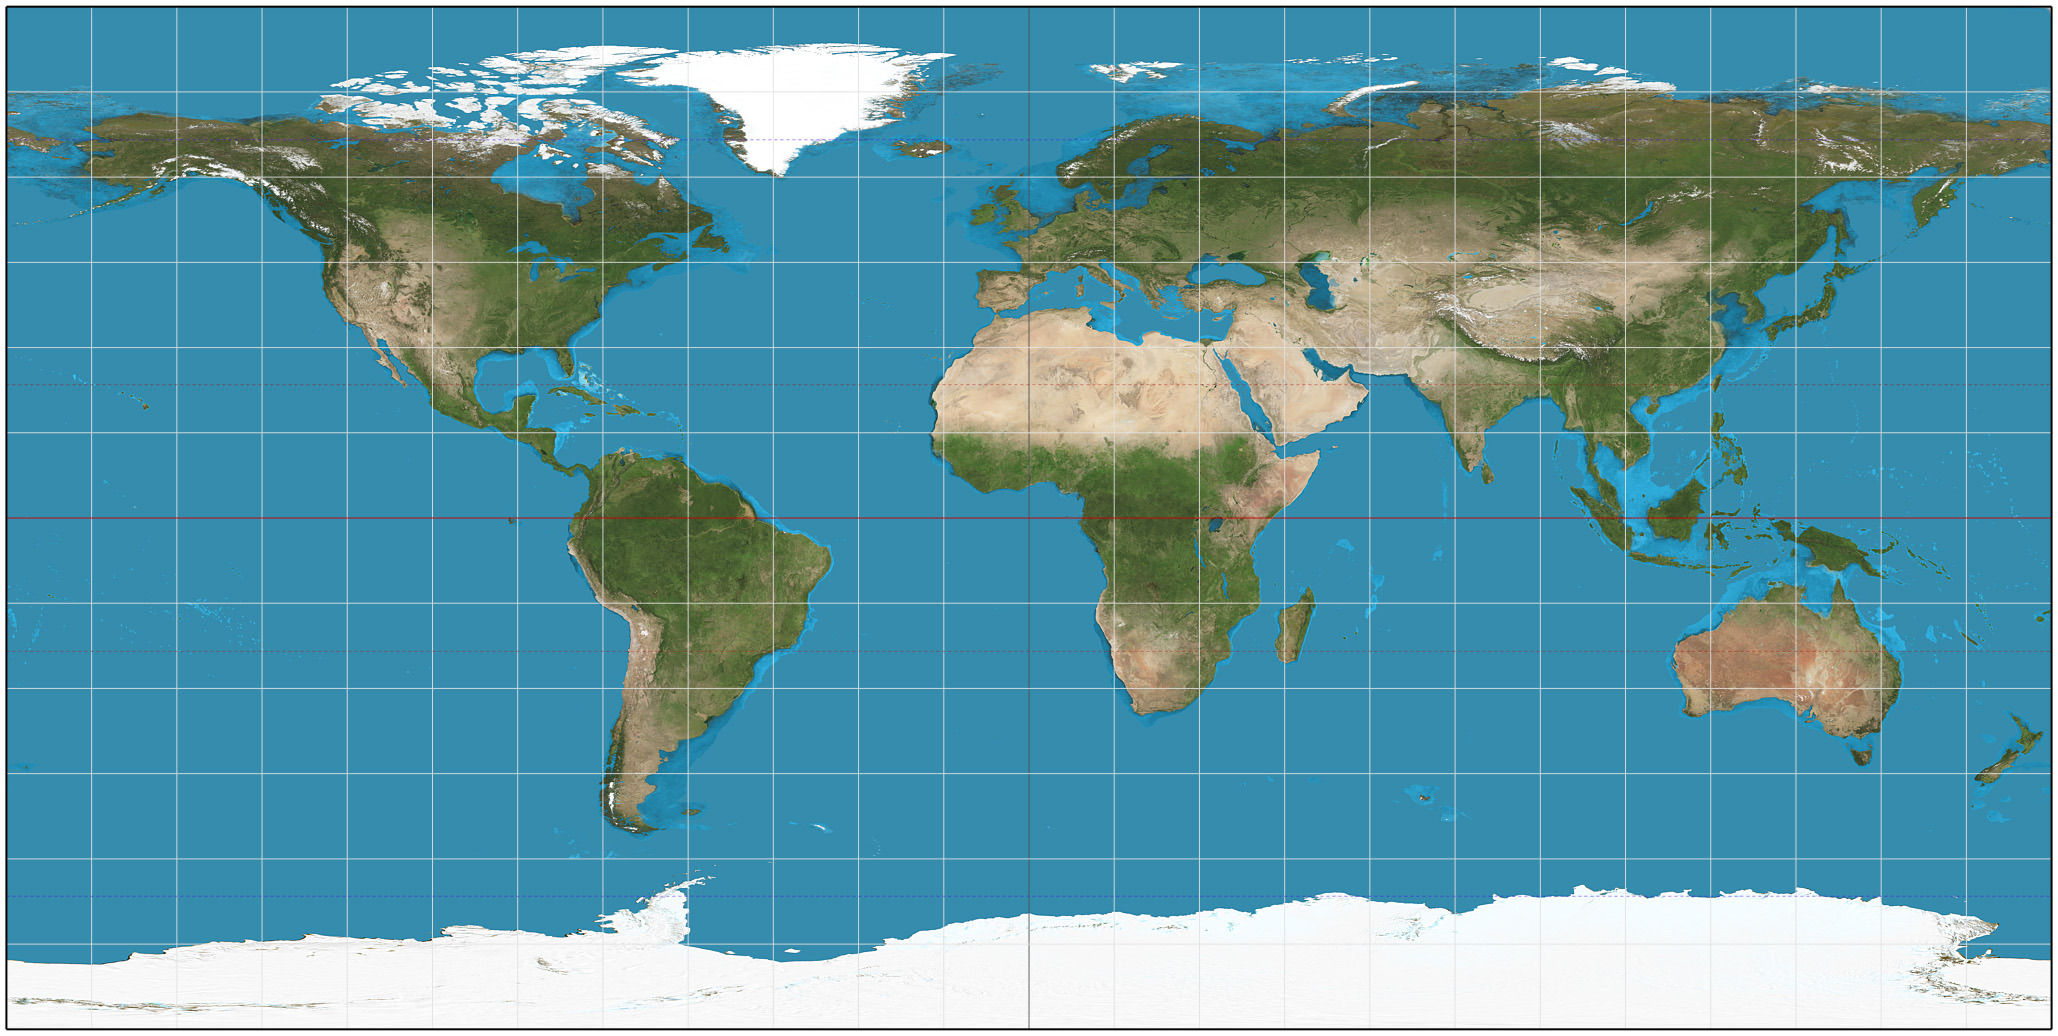
\includegraphics[width=0.6\textwidth]{media/platecaree.jpg}
\end{figure}

Note that, like all Flattening Functions, this distorts the earth -- in particular, it stretches out points near the poles, making Greenland look massive, and making Antartica look like it has more land mass than all of Asia. It also creates the illusion that, say, Canada is very far from Russia, when in truth they're very close if you go across the north pole.

\pagebreak

\section{Terminology}

OK, so you will never find the terms Globe Model and Flattening Function in the real world. Instead, you will find \emph{maddeningly} inconsistent use of terms like projection, geographic coordinate system, coordinate reference system, and projected coordinate system. Here's my attempt to summarize what these terms may mean in different contexts.



\begin{itemize}
	\item  \textbf{Projection}: Among cartographers, the term ``projection'' is synonymous with Flattening Function. All Flattening Functions are referred to as projections. But...
\begin{itemize}
	\item  In some programs (like ArcGIS), the term projection (or the term Projected Coordinate System) is used to refer to a bundle that includes \textbf{both} a Globe Model and a Flattening Model.
\end{itemize}
\item \textbf{Coordinate Reference System (CRS)}: CRS is the term used by GIS packages in R to define \textbf{both} a Globe Model and a Flattening Model.
\item \textbf{Projected Coordinate System}: The ArcGIS term for a bundle of both a Globe Model and a Flattening Model
\item \textbf{Geographic Coordinate System}: The ArcGIS term for \emph{just} a Globe Model. If you specify a Geographic Coordinate System but not a Projected Coordinate System, ArcGIS will often refuse to execute certain tools. However, it will still show you an image of your data, often by just using a \emph{Plate Carr\'ee} projection.
\end{itemize}


\section{Working with Globe Models and Flattening Functions}

Finally, note that working with different spatial datasets requires that all datasets share the same geographic coordinate system and projection. This is actually one place where ArcGIS really shines -- provided that it knows the original geographic coordinate system and projection for all data, it will reproject them on the fly, usually successfully. But be aware that if you're working in another system (like R or Python) you need to make sure all data is in the same geographic coordinate system and projection.

There are \textbf{two} things you will often have to do with projections: Define/Set the Coordinate Reference Systems, and Re-Project. Keeping straight what each of these means is one of the slipperiest concepts in GIS, so don't worry if you get confused.

\subsection{Defining or Setting your Globe Model and Flattening Function:} When you import data, what the program sees is a bunch of x-y coordinates. These x-y coordinates are just numbers. To actually be able to relate these numbers to places in the world, GIS programs need to tell the computer the Globe Model and Flattening Functions that generated those numbers.

Setting or Defining a these parameters is when you tell the program \emph{how to interpret} a set of x-y coordinates. When you set or define a these parameters, the coordinates aren't changed; you're just offering the computer information about what they mean. This may mean providing both a Globe Model and a Flattening Function (if the x-y coordinates were generated in a flattened state), or just a Globe Model (if the x-y coordinates are latitude and longitude).

In ArcGIS, you do this using the ``Define Projection'' tool; in R you do with through the command \texttt{proj4string(your\_data) = crs\_object}.

Note that you don't always have to set or define data's Globe Model and Flattening Function. If your data is in a GIS format (like a Shapefile) and came from a reputable source, it should already know its Globe Model and Flattening Function.

But many people forget to include this information, or if you're working with data in a csv, it won't be included, so you have to set these manually.

For me at least, this comes up most frequently when I import points from a csv where the coordinates are stored as latitudes and longitudes. For most modern GPS systems, in these cases you just need to set the Globe Model to what is called \texttt{WGS84}. Then remember you will need to apply a Flattening Function of your choice (see below) before analyzing your data.

When defining your the Globe Model (and possibly Flattening Function), {\color{red} there is a single correct answer}. If you tell the program to interpret the x-y coordinates it has loaded as latitude and longitude when those x-y coordinates were actually generated using a Mercator Projection, the answers you get in your analysis will be wrong.

\subsection{Applying a Flattening Function / Changing your Flattening Function:} Sometimes you have data in latitude and longitude you want to Flatten in a given way, or you've been given data that was generated using a Flattening Function that isn't the one you want to use. Changing your Flattening Function is usually referred to as ``re-projecting'' your data.

Unlike \emph{defining} a Globe Model and Flattening Function, when you re-project the x-y coordinate values in your data will actually change.

Re-projecting is only possible when you have already defined the initial geographic coordinate system / projection. This is because your GIS software knows how to convert one representation of the data to another, but it has to know both (a) what the data is now, and (b) what representation you want next. If you haven't defined at least a Globe Model, it doesn't know (a) so doesn't know what conversion to use.

Remember: when re-projecting (unlike defining), there is no such thing as the ``correct'' Globe Model and Flattening Function -- all Flattening Functions will cause distortions, and it is your job as a GIS professional to determine the Flattening Function that offers the best trade-off of distortions for your purposes.\footnote{For example, if you only care about distances, you would probably want to work with an Equidistant projection. If you care about area, you should use an equal-area projection. Etc.}

\section{Recap}\label{recap}
\begin{enumerate}
	\item Representing spatial data in two dimensions requires a Globe Model and a Flattening Function.
	\item Terms like ``projection'' often refer to Flattening Functions, but sometimes also include a Globe Model.
	\item When \emph{defining your Globe Model and Flattening Function}, it is your responsibility to determine the ``correct'' parameters based on what was used to generate the data.
	\item When \emph{re-projecting} data, there is \textbf{\emph{never}} an objectively correct set of parameters, and it is your job to choose one that fits your application.
\end{enumerate}
\end{document}
